\section{Värmeflöde genom grunden}

För att räkna på energin som flödar genom grunden är det av necessitet att räkna
transient. Detta gå berget är väldigt långsamt på att ta åt sig värme. Detta
innebär att i parktiken så uppnås aldrig ett statiskt jämviktsläge.

Problemet är behandlat med finita elementmetoden av värmeledningsekvationen.
Geometrin av problemet och trianguleringen kan ses i figur \ref{fig:foundation:tri}.
Randvärdena som är satt är att alla rander som går från berg till berg är adiabatiska.
Detta kommer inte stämma i praktiken om inte definitionsmängden sätts till oändligt
stor. För lösning av detta problem kan det dock ses som en tillräckligt god
approximation då definitionsmängden är stor och temperaturen ej varierar mycket
från förväntat värde.

Vid randerna till luft är konvektionsparametern satt
till $h = \unit[15,5]{Wm^{-2}K^{-1}}$. Detta är en siffra som motsvarar
en vindhastighet på $v = \unit[2]{ms^{-1}}$. Utomhustemperaturen har valts
som en minstakvadratanpassad trigonetrisk funktion av
medeltemperaturen de senaste tjugo åren vilket kan ses i figur
\ref{fig:foundation:meantemperature}. Anpassningen gör att
differentialekvationerna av Galerkinformuleringen kan lösas analytiskt
för alla tider istället för att systemet behöver lösas semidiskret.
Detta minskade exekveringstiden dramatiskt vilket gav möjlighet att använda en
mycket finare triangulering. Dessutom så kan alla termer i lösningen
som går mot noll då tiden går mot oändligeheten sättas till noll. Detta innebär
att få når ett transient jämviktsläge som liknar det jämviktsläge vi har i praktiken.
Initialvärdena kommer således inte ha någon betydelse och dessa kan då väljas
godtykligt. 
För att uppnå detta med semidiskret MOL behövs väldigt många itereringar för att
nå konvergens.

\begin{figure}
\centering
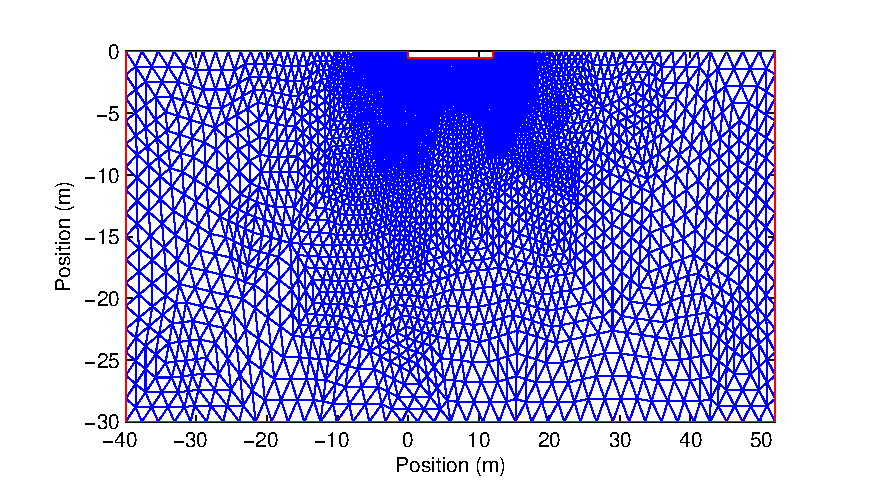
\includegraphics{images/trifoundation.eps}
\caption{Definitionsmängd samt triangulering berget under grunden.}
\label{fig:foundation:tri}
\end{figure}


\begin{figure}
\centering
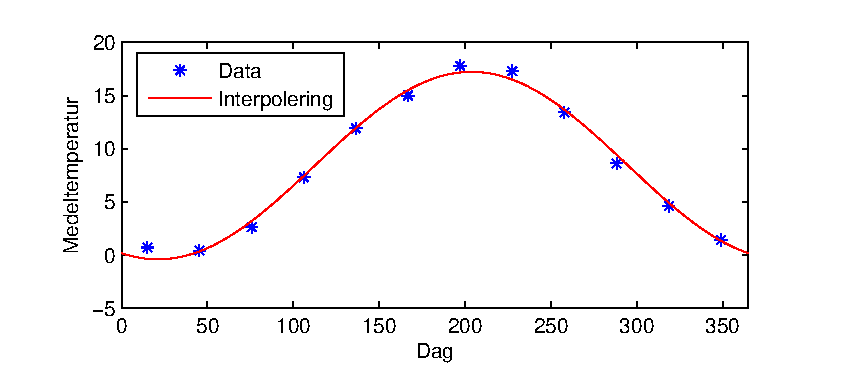
\includegraphics{images/meantemperature.eps}
\caption{
Medeltemperaturen för göteborg de senaste 20 åren. Punkterna är data tagna från Miljöförvaltningen och linjen är minstakvadratanpassningen som senare använts för att beräkna energiflöden.}
\label{fig:foundation:meantemperature}
\end{figure}

%Miljöförvaltningen
%http://www4.goteborg.se/prod%5Csk%5Cstatistik%5CstatistikR5.nsf/0/3F002A395ED39AC8C1256D3B00393D0E/$File/3.01.pdf
